% ============================================================================
% INDICON 2026 -- Paper 4422 -- revised version (v2). Single-file Overleaf main.
% The bibliography is embedded below (filecontents), so no separate .bib upload
% is needed. Upload the PDFs in the "figures" folder next to this file into a
% folder named figures/ in Overleaf. Figures are guarded with \IfFileExists,
% so the document compiles even before they are uploaded.
% Conference limit: at most 15 references -- the embedded list has exactly 15.
% ============================================================================
\begin{filecontents*}[overwrite]{references.bib}
@inproceedings{arora2026streamrag,
  author    = {Siddhant Arora and Haidar Khan and Kai Sun and Xin Luna Dong and Sajal Choudhary and Seungwhan Moon and Xinyuan Zhang and Adithya Sagar and Surya Teja Appini and Kaushik Patnaik and Sanat Sharma and Shinji Watanabe and Anuj Kumar and Ahmed A Aly and Yue Liu and Florian Metze and Zhaojiang Lin},
  title     = {Stream {RAG}: Instant and Accurate Spoken Dialogue Systems with Streaming Tool Usage},
  booktitle = {Proceedings of the 43rd International Conference on Machine Learning},
  series    = {Proceedings of Machine Learning Research},
  volume    = {306},
  pages     = {3633--3663},
  publisher = {PMLR},
  year      = {2026},
  url       = {https://proceedings.mlr.press/v306/arora26a.html}
}
@article{galbraith2026streaming,
  author    = {Elroy Galbraith},
  title     = {When Does Streaming Tool Use Help? Characterizing Tool-Intent Stabilization in Streaming Retrieval-Augmented Generation},
  journal   = {arXiv preprint arXiv:2606.20113},
  year      = {2026},
  url       = {https://arxiv.org/abs/2606.20113}
}
@article{jung2026hiding,
  author    = {Kyudan Jung and Hyunsin Park and Yoonhyung Lee and Jinhwan Park and Jinhyeok Yang and KiHyun Nam and Jaegul Choo and Jinkyu Lee},
  title     = {Hiding Tool Latency in On-Device Cascaded Voice Agent through Speculative Execution},
  journal   = {arXiv preprint arXiv:2610.07641},
  year      = {2026},
  url       = {https://arxiv.org/abs/2610.07641}
}
@inproceedings{chien2026moshirag,
  author    = {Chung-Ming Chien and Manu Orsini and Eugene Kharitonov and Neil Zeghidour and Karen Livescu and Alexandre D{\'e}fossez},
  title     = {{MoshiRAG}: Asynchronous Knowledge Retrieval for Full-Duplex Speech Language Models},
  booktitle = {Proceedings of the 43rd International Conference on Machine Learning},
  series    = {Proceedings of Machine Learning Research},
  volume    = {306},
  pages     = {19522--19545},
  publisher = {PMLR},
  year      = {2026},
  url       = {https://proceedings.mlr.press/v306/chien26b.html}
}
@article{ray2026tauvoice,
  author    = {Soham Ray and Keshav Dhandhania and Victor Barres and Karthik Narasimhan},
  title     = {$\tau$-Voice: Benchmarking Full-Duplex Voice Agents on Real-World Domains},
  journal   = {arXiv preprint arXiv:2603.13686},
  year      = {2026},
  url       = {https://arxiv.org/abs/2603.13686}
}
@inproceedings{jiang2023flare,
  author    = {Zhengbao Jiang and Frank Xu and Luyu Gao and Zhiqing Sun and Qian Liu and Jane Dwivedi-Yu and Yiming Yang and Jamie Callan and Graham Neubig},
  title     = {Active Retrieval Augmented Generation},
  booktitle = {Proceedings of the 2023 Conference on Empirical Methods in Natural Language Processing},
  pages     = {7969--7992},
  address   = {Singapore},
  publisher = {Association for Computational Linguistics},
  year      = {2023},
  doi       = {10.18653/v1/2023.emnlp-main.495}
}
@inproceedings{su2024dragin,
  author    = {Weihang Su and Yichen Tang and Qingyao Ai and Zhijing Wu and Yiqun Liu},
  title     = {{DRAGIN}: Dynamic Retrieval Augmented Generation based on the Real-time Information Needs of Large Language Models},
  booktitle = {Proceedings of the 62nd Annual Meeting of the Association for Computational Linguistics (Volume 1: Long Papers)},
  pages     = {12991--13013},
  address   = {Bangkok, Thailand},
  publisher = {Association for Computational Linguistics},
  year      = {2024},
  doi       = {10.18653/v1/2024.acl-long.702}
}
@inproceedings{jeong2024adaptiverag,
  author    = {Soyeong Jeong and Jinheon Baek and Sukmin Cho and Sung Ju Hwang and Jong Park},
  title     = {{Adaptive-RAG}: Learning to Adapt Retrieval-Augmented Large Language Models through Question Complexity},
  booktitle = {Proceedings of the 2024 Conference of the North American Chapter of the Association for Computational Linguistics: Human Language Technologies (Volume 1: Long Papers)},
  pages     = {7036--7050},
  address   = {Mexico City, Mexico},
  publisher = {Association for Computational Linguistics},
  year      = {2024},
  doi       = {10.18653/v1/2024.naacl-long.389}
}
@inproceedings{moskvoretskii2025adaptive,
  author    = {Viktor Moskvoretskii and Maria Marina and Mikhail Salnikov and Nikolay Ivanov and Sergey Pletenev and Daria Galimzianova and Nikita Krayko and Vasily Konovalov and Irina Nikishina and Alexander Panchenko},
  title     = {Adaptive Retrieval Without Self-Knowledge? Bringing Uncertainty Back Home},
  booktitle = {Proceedings of the 63rd Annual Meeting of the Association for Computational Linguistics (Volume 1: Long Papers)},
  pages     = {6355--6384},
  address   = {Vienna, Austria},
  publisher = {Association for Computational Linguistics},
  year      = {2025},
  doi       = {10.18653/v1/2025.acl-long.319}
}
@article{kadavath2022language,
  author    = {Saurav Kadavath and Tom Conerly and Amanda Askell and Tom Henighan and Dawn Drain and Ethan Perez and Nicholas Schiefer and Zac Hatfield-Dodds and Nova DasSarma and Eli Tran-Johnson and Scott Johnston and Sheer El-Showk and Andy Jones and Nelson Elhage and Tristan Hume and Anna Chen and Yuntao Bai and Sam Bowman and Stanislav Fort and Deep Ganguli and Danny Hernandez and Josh Jacobson and Jackson Kernion and Shauna Kravec and Liane Lovitt and Kamal Ndousse and Catherine Olsson and Sam Ringer and Dario Amodei and Tom Brown and Jack Clark and Nicholas Joseph and Ben Mann and Sam McCandlish and Chris Olah and Jared Kaplan},
  title     = {Language Models (Mostly) Know What They Know},
  journal   = {arXiv preprint arXiv:2207.05221},
  year      = {2022},
  doi       = {10.48550/arXiv.2207.05221}
}
@inproceedings{mallen2023trust,
  author    = {Alex Mallen and Akari Asai and Victor Zhong and Rajarshi Das and Daniel Khashabi and Hannaneh Hajishirzi},
  title     = {When Not to Trust Language Models: Investigating Effectiveness of Parametric and Non-Parametric Memories},
  booktitle = {Proceedings of the 61st Annual Meeting of the Association for Computational Linguistics (Volume 1: Long Papers)},
  pages     = {9802--9822},
  address   = {Toronto, Canada},
  publisher = {Association for Computational Linguistics},
  year      = {2023},
  doi       = {10.18653/v1/2023.acl-long.546}
}
@inproceedings{yang2018hotpotqa,
  author    = {Zhilin Yang and Peng Qi and Saizheng Zhang and Yoshua Bengio and William Cohen and Ruslan Salakhutdinov and Christopher D. Manning},
  title     = {{HotpotQA}: A Dataset for Diverse, Explainable Multi-hop Question Answering},
  booktitle = {Proceedings of the 2018 Conference on Empirical Methods in Natural Language Processing},
  pages     = {2369--2380},
  address   = {Brussels, Belgium},
  publisher = {Association for Computational Linguistics},
  year      = {2018},
  doi       = {10.18653/v1/D18-1259}
}
@inproceedings{ekstedt2022vap,
  author    = {Erik Ekstedt and Gabriel Skantze},
  title     = {Voice Activity Projection: Self-supervised Learning of Turn-taking Events},
  booktitle = {Proc. Interspeech 2022},
  pages     = {5190--5194},
  year      = {2022},
  doi       = {10.21437/Interspeech.2022-10955}
}
@inproceedings{bohus2011decisions,
  author    = {Dan Bohus and Eric Horvitz},
  title     = {Decisions about turns in multiparty conversation: from perception to action},
  booktitle = {Proceedings of the 13th International Conference on Multimodal Interfaces (ICMI '11)},
  pages     = {153--160},
  address   = {Alicante, Spain},
  publisher = {ACM},
  year      = {2011},
  doi       = {10.1145/2070481.2070507}
}
@article{howard1966information,
  author    = {Ronald A. Howard},
  title     = {Information Value Theory},
  journal   = {IEEE Transactions on Systems Science and Cybernetics},
  volume    = {2},
  number    = {1},
  pages     = {22--26},
  year      = {1966},
  doi       = {10.1109/TSSC.1966.300074}
}
\end{filecontents*}

\documentclass[conference]{IEEEtran}
\IEEEoverridecommandlockouts

\usepackage{cite}
\usepackage{amsmath,amssymb,amsfonts,amsthm}
\usepackage{algorithm}
\usepackage[noend]{algpseudocode}
\usepackage{graphicx}
\usepackage{textcomp}
\usepackage{xcolor}
\usepackage{fancyhdr}
\usepackage[hidelinks]{hyperref}  % hidelinks: no green/red boxes around citations and references
\usepackage{placeins}              % \FloatBarrier: keeps tables/figures from drifting past the references
\usepackage{booktabs}
\usepackage{multirow}
\usepackage{url}
\graphicspath{{figures/}}

\newtheorem{proposition}{Proposition}
\newtheorem{corollary}{Corollary}

% Notation used in the tables and theory (one spelling everywhere).
\newcommand{\Bplus}{B9\textsuperscript{+}}
\newcommand{\Bten}{B10}
\newcommand{\Beleven}{B11}
\newcommand{\DC}{\Delta_{\mathrm{C}}}
\newcommand{\DS}{\Delta_{\mathrm{S}}}
\newcommand{\lamL}{\lambda_l}
\newcommand{\lamC}{\lambda_c}
\newcommand{\pol}[1]{\texttt{#1}}
\newcommand{\dset}[1]{\texttt{#1}}

% Starts a new row of authors (3 authors per row).
\makeatletter
\newcommand{\linebreakand}{%
  \end{@IEEEauthorhalign}
  \hfill\mbox{}\par
  \mbox{}\hfill\begin{@IEEEauthorhalign}
}
\makeatother

\def\BibTeX{{\rm B\kern-.05em{\sc i\kern-.025em b}\kern-.08em
    T\kern-.1667em\lower.7ex\hbox{E}\kern-.125emX}}

\fancypagestyle{firstpage}{
  \fancyhf{}
  \fancyhead[C]{23rd Edition of IEEE India Council International Conference (INDICON 2026)}
  \fancyfoot[L]{%
      \begin{minipage}[t]{\textwidth}
      \normalsize{979-8-3195-2581-9/26/\$31.00 \copyright2026 IEEE}
    \end{minipage}%
  }
  \renewcommand{\headrulewidth}{0pt}
}

\pagestyle{fancy}
\fancyhf{}
\fancyfoot[C]{INDICON 2026}
\renewcommand{\headrulewidth}{0pt}

\begin{document}

\title{Joint vs. Decomposed Control of Retrieval and Timing in Streaming Voice RAG}

\author{
\IEEEauthorblockN{Renya Peter}
\IEEEauthorblockA{\textit{Information Science and Engineering}\\
\textit{Ramaiah Institute of Technology}\\
Bengaluru, India\\
\texttt{renya.peter@gmail.com}}
\and
\IEEEauthorblockN{Ryan Gomez}
\IEEEauthorblockA{\textit{Electronics and}\\
\textit{Communication Engineering}\\
\textit{Ramaiah Institute of Technology}\\
Bengaluru, India\\
\texttt{ryangomez9965@gmail.com}}
\and
\IEEEauthorblockN{Shubhankit Singh}
\IEEEauthorblockA{\textit{Computer Science and}\\
\textit{Engineering (AI/ML)}\\
\textit{Ramaiah Institute of Technology}\\
Bengaluru, India\\
\texttt{shubhankitsingh20@gmail.com}}
\linebreakand
\IEEEauthorblockN{Lakshya Jaiswal}
\IEEEauthorblockA{\textit{Computer Science and Engineering}\\
\textit{Ramaiah Institute of Technology}\\
Bengaluru, India\\
\texttt{lakjai0707@gmail.com}}
\and
\IEEEauthorblockN{Adithi Nellukuduri Borannavara}
\IEEEauthorblockA{\textit{Information Science and Engineering}\\
\textit{BMS Institute of Technology}\\
\textit{and Management}\\
Bengaluru, India\\
\texttt{adithinb047@gmail.com}}
\and
\IEEEauthorblockN{Yashmita Sudhir}
\IEEEauthorblockA{\textit{Electronics and}\\
\textit{Communication Engineering}\\
\textit{Ramaiah Institute of Technology}\\
Bengaluru, India\\
\texttt{yashmita.sudhir@gmail.com}}
}

\IEEEaftertitletext{\vspace{-1.5\baselineskip}}% pulls the abstract up under the author block
\maketitle
\thispagestyle{firstpage}

\begin{abstract}
A streaming voice dialogue system must decide whether to retrieve external
knowledge and when to dispatch the query while the user is still speaking. We
ask whether optimizing these two decisions jointly outperforms a decomposed
controller that faces the same latency and compute prices. Under
timing-invariant quality, constant latency overlap and a dispatch-invariant
belief (A1--A3), we prove that the joint controller makes the same retrieval
decisions as a decomposed controller at a mapped price, and that a decomposed
controller pricing the expected exposed latency is identical to it. Without
these assumptions, coupling can help mainly when the belief sharpens during
the turn and a dispatched retrieval is committed. We then ran a
pre-registered test on open-domain and customer-support speech with live
automatic speech recognition (ASR) partials. On 3,734 open-domain test
questions the joint controller was worse than the strongest decomposed rival
under commitment (utility difference $-0.037$, 95\% CI $[-0.048,-0.025]$):
the boundary hypotheses were not supported and the pre-registered reverse
hypothesis held. Customer-support and pooled results point the same way but
are exploratory. The gap disappears on clean text, which points to
recognition errors in early partial transcripts and a weak belief signal.
\end{abstract}
\begin{IEEEkeywords}
Retrieval-Augmented Generation, Spoken Dialogue Systems, Decision-Theoretic Control, Speculative Prefetch, Streaming Retrieval.
\end{IEEEkeywords}


% =============================================================================
\section{Introduction}\label{sec:intro}

A voice assistant that grounds answers in external documents must decide whether to retrieve on a turn and when to dispatch retrieval relative to ongoing speech. Streaming systems already retrieve mid-speech, either speculatively at fixed intervals or when triggered by the model, and reduce latency without losing accuracy \cite{arora2026streamrag,jung2026hiding}. Retrieval is not always beneficial, however. Adaptive methods decide whether to search \cite{jiang2023flare,su2024dragin,jeong2024adaptiverag}, and retrieved documents can degrade answers the language model would otherwise get right \cite{mallen2023trust}. Work on timing typically dispatches once user intent stabilizes and assumes retrieval is required \cite{galbraith2026streaming}. As a result, the two decisions are studied as separate problems.

This raises an architectural question: must the two decisions be made jointly by a coupled controller, or does a decomposed controller facing the same latency and compute prices perform equally well? In a controlled text-based experiment, a coupled controller strictly dominated a price-aware decomposed baseline in 0 of 5 seeds (Section~\ref{sec:res-equiv}). We show this is not a matter of statistical power: when the timing and belief assumptions A1--A3 hold, the joint controller's retrieval decisions are those of a decomposed controller at a different price. We formalize this equivalence and identify the conditions under which the two architectures can diverge.

Our approach builds on uncertainty-triggered retrieval \cite{jiang2023flare,su2024dragin}, speculative dispatch on partial transcripts \cite{arora2026streamrag,jung2026hiding}, and internal knowledge probing \cite{kadavath2022language,moskvoretskii2025adaptive}. We make three contributions:
\begin{itemize}
    \item \textbf{Theory:} to our knowledge, the first formal equivalence analysis of joint and decomposed retrieval control: an exact price map and gap bound under A1--A3 (Props.~\ref{prop:eq}--\ref{prop:gap}), and the violations of A1--A3 that can separate the two.
    \item \textbf{Streaming test:} a pre-registered comparison on live ASR partials under committed and speculative retrieval.
    \item \textbf{Diagnostics and data:} a price-aware objective with measured retrieval harm, an analysis of beliefs on partial transcripts, and a matched-pair spoken customer-support benchmark. Data, code and protocol are public.\footnote{\url{https://github.com/SOYL-AI/voice-rag-controller} (tag \texttt{v2-final}).}
\end{itemize}

\section{Related Work}\label{sec:related}

\textbf{Streaming and speculative retrieval.} Stream RAG issues retrieval and
tool calls while the user is still speaking, either speculatively at fixed
intervals or when triggered by the model \cite{arora2026streamrag}; these
correspond to our speculative and commit architectures. Speculative execution
also hides tool latency in on-device voice agents \cite{jung2026hiding}.
Galbraith studies when tool intent stabilizes on a streaming transcript, but
considers timing alone and assumes every query needs retrieval
\cite{galbraith2026streaming}. MoshiRAG learns whether to retrieve in a
full-duplex speech model, but retrieves only at response onset
\cite{chien2026moshirag}. To our knowledge, none asks whether the two
decisions should be made jointly under shared prices.

\textbf{Adaptive retrieval and self-knowledge.} FLARE and DRAGIN trigger
retrieval from generation uncertainty \cite{jiang2023flare,su2024dragin},
Adaptive-RAG routes queries by predicted complexity \cite{jeong2024adaptiverag},
and simple uncertainty triggers remain competitive
\cite{moskvoretskii2025adaptive}. Models can predict whether they know an
answer \cite{kadavath2022language}; our probe belongs to this family.
Retrieval can also hurt on questions the model already answers correctly
\cite{mallen2023trust}, which motivates the harm term $g^{-}$.

\textbf{Datasets and decision theory.} We draw open-domain questions from
PopQA \cite{mallen2023trust} and HotpotQA \cite{yang2018hotpotqa}. Value of
information \cite{howard1966information} and decision-theoretic turn-taking
\cite{bohus2011decisions} underlie our objective; what is new is an exact
account of when joint and decomposed control coincide.

% =============================================================================
\section{Problem Formulation and Controllers}
\label{sec:problem}

\subsection{Problem Formulation}
\label{subsec:problem_formulation}

While the user speaks, a streaming recogniser emits partial transcripts
$x_1,\dots,x_K$; $x_K$ is the transcript at the voice-activity (VAD) end of
turn. For each turn the assistant decides \emph{whether} to retrieve
documents or answer closed-book, and \emph{when} to send the retrieval
request. A request sent during speech overlaps the remaining speech and hides
part of its latency, but it is built from an incomplete question. After each
partial the system updates a belief $b_k$ that the turn needs retrieval and a
prediction $\hat R_k$ of the remaining speech. The controller then
dispatches, waits, or (at the end of the turn) skips. Passages go to the
generator (Mistral-7B), whose answer is spoken by TTS. User-perceived delay
is the time to first audio,
$\mathrm{TTFA}=t_{\text{first audio}}-t_{\text{user end}}$.
All controllers maximise the same priced objective
(Section~\ref{subsec:priced_objective}); they differ only in whether the two
decisions are made jointly or by separate modules
(Section~\ref{subsec:decision_rule}). Fig.~\ref{fig:system_flow} shows the
pipeline and the three decision structures we compare.

\begin{figure*}[t]
\centering
\IfFileExists{figures/fig_framework.pdf}{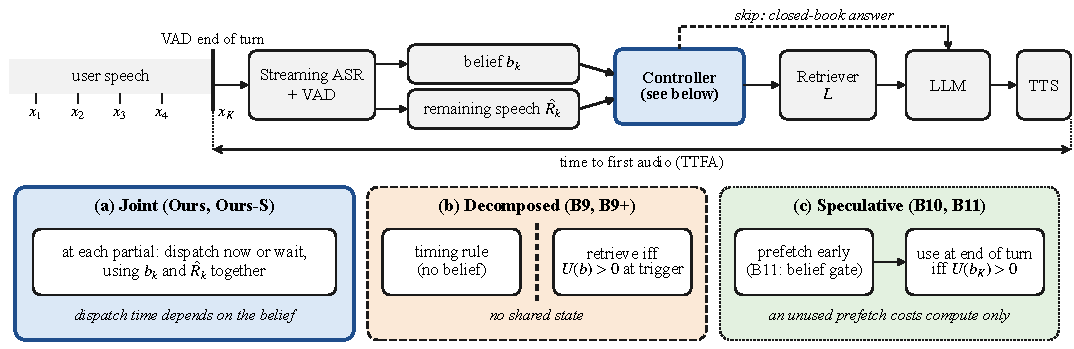
\includegraphics[width=\textwidth]{fig_framework.pdf}}{\fbox{Upload figures/fig\_framework.pdf}}
\caption{Streaming pipeline and the decision structures compared. From each
ASR partial $x_k$ the system estimates the belief $b_k$ and the remaining
speech $\hat R_k$; the controller dispatches a retrieval or answers
closed-book. The decision rules are given by Eq.~(\ref{eq:obj}) and
Algorithm~\ref{alg:oursv2}.}
\label{fig:system_flow}
\end{figure*}

\subsection{Belief State}
\label{subsec:belief_state}

\textit{Text experiment.} The belief is computed once per turn from the full
question $q$: the signal is the mean per-token entropy (nats) of a closed-book
draft, averaged over five drafts,
\begin{equation}
\begin{aligned}
s&=\frac{1}{N}\sum_{i=1}^{N}H\!\left(p_\theta(\cdot\mid y_{<i},q)\right),\\
b&=\max\!\big(0.05,\,\sigma(ws+c)\big),
\end{aligned}
\label{eq:belief}
\end{equation}
with $w=11.288$, $c=-3.633$ fitted in-sample on the 36-item belief set
(180 samples, five seeds). Maximum entropy ranked these items slightly
better (AUC 0.978 vs.\ 0.925), but the mean is smoother and suits a logistic
fit; we did not run a separate controller on the maximum-entropy signal.
Because it is computed once from the full question, this belief does not
depend on dispatch time.

\textit{Streaming experiment.} The belief is recomputed on every partial
$x_k$. Mistral-7B is asked whether the question can be answered from general
knowledge alone, without the organisation's own information; the signal is
the probability it gives to ``No'' (one generated token). It is calibrated per
dataset on the development split only, as a logistic function of the
signal's logit, the fraction of the question heard, and their interaction.
An item needs retrieval when its closed-book answer is wrong in at least
three of five drafts.

\subsection{Actions and Dispatch Timing}
\label{subsec:action_space}

In the text experiment the action is skip or retrieve with one of three
timing rules on text read at 150 words per minute: \textsc{sentence\_end}
dispatches when the question ends; \textsc{immediate} at the first partial
after the prefix becomes query-ready at $t_{\text{ready}}$ (four words, one of
them a content word); and \textsc{fixed\_early\_proxy} at
$\max(\min(0.35T,0.8t_1),t_{\text{ready}})$, where $T$ is the question's
duration and $t_1$ the time of the first partial. Neither early rule forecasts the end of the turn. In the
streaming experiment the controller may dispatch at any partial, so timing
becomes an optimal-stopping problem. We test two architectures on the same
items and prices: under \textsc{commit} a dispatched retrieval is always used;
under \textsc{speculative} it may be discarded at the end of the turn, at the
cost of its compute.

\subsection{Latency- and Compute-Priced Objective}
\label{subsec:priced_objective}

Retrieving with belief $b$, dispatched at $t$, has utility
\begin{equation}
U_t(b)=b\,g^{+}(1-\rho_t)-(1-b)\,g^{-}-\lambda_l e_t-\lambda_c(1+w_t),
\label{eq:obj}
\end{equation}
and skipping has $U(\text{skip})=0$. Here $g^{+}$ is the accuracy gained by
retrieving on turns that need it, $g^{-}$ the accuracy lost on turns that do
not, $\rho_t$ the share of $g^{+}$ lost to a partial query,
$\rho(t)=1-\text{hit@3}(t)/\text{hit@3}(\text{end})$, $e_t$ the exposed
latency (s), $w_t$ the expected wasted retrievals, and $\lambda_l$,
$\lambda_c$ the prices of latency and compute in accuracy units.

A common simplification sets $g^{+}=1$, $g^{-}=\rho_t=0$, i.e.\ it uses $b$
itself as the gain and assumes retrieval never hurts. In the text experiment
retrieval added $g^{+}=0.720$ [0.504, 0.888] on needed turns but cost
$g^{-}=0.592$ [0.408, 0.768] on the others, so at zero prices one should
retrieve only when $b>g^{-}/(g^{+}+g^{-})=0.451$, not when $b>0.05$. In the
streaming experiment, $g^{\pm}$ are estimated on the development split:
$\hat g^{+}=0.441$, $\hat g^{-}=-0.112$ on \dset{d1\_open} (retrieval did not
hurt) and $0.445$, $0.034$ on \dset{d2\_support}.

With fixed timing policies the exposure is $e_t=L-o_t$, with a fixed overlap
$o_t$ per policy. In the streaming experiment it depends on the turn,
\begin{equation}
e_k=\mathbb{E}_L\!\left[\max(0,\ L-W_k)\right]+\pi,
\label{eq:exposure}
\end{equation}
where $L$ is the latency of the retrieval call itself (query rewriting plus
search), $W_k=\hat R_k+d$ the predicted remaining speech plus the end-of-turn
detection delay $d$ ($d=0$ here; the turn ends at the VAD endpoint), and
$\pi$ the rest of retrieval's cost to TTFA, which no timing can hide: the
longer prompt's prefill and the generation and synthesis up to the first
spoken clause ($\pi=371$~ms on the development split). Dispatching at the end
of the turn therefore costs $\mathbb E[L]+\pi$. The waste term $w_t$ is not
measured in either experiment: the text experiment uses fixed placeholders
(0.02 and 0.08 for the two early policies, 0 at sentence end), and the
streaming experiment uses $w(f)=0.1(1-f)$ for a dispatch made with a fraction
$f$ of the question heard ($w=0$ at the end of the turn). It enters only the
decision; the scored utility charges $\lambda_c$ per dispatched retrieval.
Section~\ref{sec:res-secondary} reports a sensitivity check over
$w\in\{0,0.04,0.08,0.16\}$. We fix $\lambda_c=0.05$. The text experiment
sweeps $\lambda_l$; the streaming test uses one pre-registered price per
dataset, $\lambda_l=0.173$ (\dset{d1\_open}) and $0.216$ (\dset{d2\_support})
per second.

\subsection{Controllers}
\label{subsec:decision_rule}

Table~\ref{tab:controllers} lists the controllers. All priced controllers
share Eq.~(\ref{eq:obj}), the belief calibration, the remaining-speech
predictor, the latency model and $g^{\pm}$. In the streaming experiment all
baseline thresholds and timing rules are tuned on the development split with
an equal budget (the text experiment used fixed defaults).

\textbf{Ours} (text experiment) scores skip and every (retrieve, $t$) pair
and takes the best. \textbf{B9} splits the choice into a timing module and a
retrieval module that share no state, so it prices retrieval at the full
latency $L$ and can skip turns that early dispatch would make worthwhile.
Unlike B8, which retrieves on a fixed entropy threshold with a fixed early
dispatch, B9 prices both decisions (Algorithm~\ref{alg:oursv2}). \textbf{B9+}
keeps the split but prices the expected exposure of its own timing choice. In
the streaming experiment its timing rule is chosen on the development split
from four families (early, late, a threshold on $\hat R$, and dispatch once
$\hat R$ falls below a threshold). The selected rule dispatches at the first
query-ready partial whose predicted remaining speech is at most 698~ms
(\dset{d1\_open}) or 649~ms (\dset{d2\_support}) at the primary price.

\textbf{Ours-S} (streaming) compares, at each partial, the value of
dispatching now, $U_k(b_k)$, with the value of waiting one more partial.
Beliefs are discretised into ten bins, and transition matrices
$P(b'\mid b,\phi)$ for three phases of the utterance ($\phi$ = fraction heard,
split at 0.34 and 0.67) are fitted on development sequences. The next partial
arrives after the development-median gap $s$ and brings new information with
probability $p=P(R>s)$ under the predicted remaining-speech quantiles;
otherwise the next step is the end of the turn. With lookahead depth one,
\begin{equation}
\textsc{Wait}=p\,\mathbb E\big[\max\big(U_{k+1}(b'),V_{\mathrm{end}}(b')\big)\big]+(1-p)\,V_{\mathrm{end}}(b_k),
\label{eq:wait}
\end{equation}
where $V_{\mathrm{end}}(b)=\mathbb E[\max(U_K(b''),0)\mid b]$ and $U_K$ is
Eq.~(\ref{eq:obj}) with $W=0$ and $\rho=w=0$. At the end of the turn Ours-S
retrieves iff $U_K>0$. It has no tuned parameter beyond the shared models,
and the depth was fixed before the test. Under \textsc{speculative} the same
rule values having the passages ready. \textbf{B10} (SPEC) always prefetches
at its trigger and uses the passages only if $U(b_K)>0$; \textbf{B11}
(SPEC-$\theta$) prefetches only when a belief-only estimate says the prefetch
is worth it. Both use a development-tuned trigger.

\begin{table}[t]
\caption{Controllers. ``Priced'': reads $(\lambda_l,\lambda_c)$. ``Joint'':
whether and when chosen in one decision.}
\label{tab:controllers}
\centering
\footnotesize
\setlength{\tabcolsep}{3pt}
\begin{tabular}{@{}l p{4.1cm} c c@{}}
\toprule
ID & Rule & Priced & Joint\\
\midrule
B0 & never retrieve & -- & --\\
B4 & $1-\bar p\ge0.5$ (FLARE-style~\cite{jiang2023flare}); sentence end & no & no\\
B6 & $s^{\max}\ge1.0$ (DRAGIN-style~\cite{su2024dragin}); sentence end & no & no\\
B8 & $s^{\max}\ge1.2$; fixed early dispatch & no & no\\
B9 & Eq.~(\ref{eq:obj}) at full latency; timing separate & yes & no\\
B9+ & Eq.~(\ref{eq:obj}) at expected exposure of own timing & yes & no\\
B10 & always prefetch; use iff $U(b_K)>0$ (streaming) & yes & no\\
B11 & B10 with a belief gate on prefetch (streaming) & yes & no\\
Ours & $\arg\max$ over skip and $(\text{retrieve},t)$ (text) & yes & yes\\
Ours-S & optimal stopping over partials (streaming) & yes & yes\\
\bottomrule
\end{tabular}
\end{table}

\begin{algorithm}[t]
\caption{Ours-S (\textsc{commit}) and the decomposed B9, one turn}
\label{alg:oursv2}
\begin{algorithmic}[1]
\Statex \textbf{Ours-S (joint, streaming)}
\For{each partial $k$ as it arrives}
  \State $u\gets U_k(b_k)$ \Comment{Eqs.~(\ref{eq:obj}), (\ref{eq:exposure})}
  \If{$k=K$} \Return \textsc{Retrieve} \textbf{if} $u>0$ \textbf{else} \textsc{Skip}
  \EndIf
  \If{$u>0$ \textbf{and} $u\ge\textsc{Wait}$} \Return \textsc{Retrieve} \Comment{Eq.~(\ref{eq:wait})}
  \EndIf
\EndFor
\Statex \textbf{B9 (decomposed, text experiment)}
\State $\tau\gets\arg\max_t[\lambda_l o_t-\lambda_c w_t]$ \Comment{timing; no belief}
\State $r\gets\mathbf 1\{b g^{+}-(1-b)g^{-}-\lambda_l L-\lambda_c(1+w_{\mathrm{se}})>0\}$ \Comment{full $L$}
\State \Return $(r,\tau)$
\end{algorithmic}
\end{algorithm}

% =============================================================================
\section{Theory}\label{sec:theory}
Joint and decomposed control can differ only through what one controller sees
and the other does not; the three assumptions below remove every such
difference. The text experiment meets them by design: it retrieves with a
frozen query, uses one overlap per timing policy (0, 0.050 and 0.188~s), and
computes the belief once from the full question. Proofs are in the repository.

Write $\kappa_t=\lambda_l e_t+\lambda_c(1+w_t)$, so that
$U_t(b)=b\,g^{+}(1-\rho_t)-(1-b)\,g^{-}-\kappa_t$. The equivalence regime assumes
\textbf{(A1)} $\rho_t\equiv\bar\rho$;
\textbf{(A2)} $e_t$ is constant across turns;
\textbf{(A3)} one belief per turn, independent of dispatch time.
Under (A1) every slope is $s=g^{+}(1-\bar\rho)+g^{-}$. Let
$t^{*}=\arg\min_t\kappa_t$, $c_O=\kappa_{t^{*}}$ and
$\lambda_l'=[c_O-\lambda_c(1+w_{\mathrm{se}})]/L$.

\begin{proposition}[Equivalence]\label{prop:eq}
Assume (A1)--(A3) and $w_{\mathrm{se}}=\min_tw_t$. For every $b\in[0,1]$, Ours
at $(\lambda_l,\lambda_c)$ retrieves iff B9 at $(\lambda_l',\lambda_c)$
retrieves. The map $\lambda_l\mapsto\lambda_l'$ is a continuous, strictly
increasing bijection of $[0,\infty)$. When the maximal-overlap timing is optimal,
\[
\lambda_l'=\lambda_l\frac{L-o^{*}}{L}+\lambda_c\frac{w^{*}-w_{\mathrm{se}}}{L}.
\]
Conditional on retrieving, the timings coincide unless $\lambda_l$ and
$\lambda_l'$ lie in different linear pieces of $\lambda\mapsto\min_t\kappa_t$.
\end{proposition}
Proposition~\ref{prop:eq} says that, under A1--A3, the joint controller's
retrieval decisions are exactly those of B9 at a lower latency price. The
timings also match, except at prices where $\lambda_l$ and $\lambda_l'$ fall
in different linear pieces; outside those intervals the two controllers have
the same operating points. The stronger statement is the last line of
Proposition~\ref{prop:gap}: B9+, which keeps the decomposition but prices the
expected exposure of its own timing, decides exactly as the joint controller
at the same price.

\begin{proposition}[Gap at a fixed price]\label{prop:gap}
Assume (A1)--(A3) and model correctness: $\mathbb E[N\mid b]=b$, and realized
quality, latency and compute in expectation equal to those in
Eq.~(\ref{eq:obj}). Let $c_B=\lambda_lL+\lambda_c(1+w_{\mathrm{se}})$ and
$\mathcal B=(\theta_O,\theta_B]$ with $\theta_O=(c_O+g^{-})/s$ and
$\theta_B=(c_B+g^{-})/s$. Then
\begin{align*}
0\le\mathbb E[U_{\mathrm{Ours}}-U_{\mathrm{B9}}]
&\le(c_B-c_O)\Pr(b\in\mathcal B)\\
&\le\lambda_lo^{*}\Pr(b\in\mathcal B).
\end{align*}
For B9+ at the same price the difference is $0$ pointwise.
\end{proposition}
At a fixed price the two controllers differ only for beliefs inside the band
$\mathcal B$, and the expected gain is at most the hidden latency, priced,
times the probability of landing in the band. The bound holds under the
controller's own model. If the model is wrong, for example if retrieval costs
more latency than assumed, the realized gap can be negative.

\textbf{Channels that break the equivalence.} Each assumption can be dropped
on its own. Without (A2) (turn-dependent overlap), the gain over B9+ comes
only from variation in exposure among turns with the same belief; if the
belief has a continuous density and that variation is small, the gain scales
as $\lambda_l^{2}\operatorname{Var}e^{*}$ and is correspondingly small. Without (A1)
alone (partial-query risk), the optimal timing depends on $b$, but the joint
optimum is still a function of $b$, so the two classes do not separate.
Without (A3), the belief sharpens as speech arrives. For a committed
retrieval with value $D_k$ at partial $k$, waiting is worth
$W_k=\mathbb E[D_{k+1}^{+}\mid\mathcal F_k]-D_k^{+}$. If turns that a
belief-free timing rule cannot tell apart include both turns with $W_k>0$ and
turns where dispatching now is strictly better, every decomposed policy is
strictly suboptimal, and this gain does not rely on the exposure varying.
Under speculative prefetch, the joint gain over always-prefetch (B10) is at
most the compute spent on prefetches the joint controller would skip plus a
partial-query term, and with two decision points a belief-gated prefetcher
(B11) comes within a term of the same size as the (A2) gain. These
predictions define the pre-registered tests: P1, joint beats \Bplus{} under
commit ($\DC>0$); P2, the advantage shrinks under speculation
($\DC-\DS>0$); P3, under speculation the joint controller is within
$m_3=0.016$ of the best decomposed rival (equivalence test); and H-REV,
$\DC<0$, added before the freeze because the development data pointed that
way. The boundary claim requires P1, P2 and P3 together.

% =============================================================================
\section{Experimental Setup}\label{sec:setup}
\textbf{Model and retrieval.} All controllers use the same generator,
Mistral-7B-Instruct-v0.3 served with vLLM, and the same retriever, a FAISS
index over bge-small embeddings. Every item is run with five seeds (11, 23, 37,
53 and 71), which change only the generator's sampling; seeds are therefore
not independent replicates, and the unit of analysis is the item.

\textbf{Text experiment.} To check the equivalence result we use 50
single-domain (hotel) scenarios, each run with the five seeds, and a set of
36 items (two shared with the scenarios) to validate the belief signal.
Questions are revealed as text at 150 words per minute, and the setup meets
A1--A3 by construction (Section~\ref{sec:theory}).

\textbf{Streaming datasets.} \dset{d1\_open} combines popularity-stratified
PopQA \cite{mallen2023trust} with multi-hop HotpotQA \cite{yang2018hotpotqa}:
5,300 items, 1,566 for development and 3,734 for test. \dset{d2\_support} is a
customer-support set of 720 items covering 12 domains and 24 fictional
organisations (222 development, 498 test). Its questions are built in matched
groups, some needing the organisation's own documents and some answerable from
general knowledge, so that need cannot be read from the wording; a
surface-form classifier reaches only AUC 0.576 [0.541, 0.617].

\textbf{Speech.} Each item is synthesised with one Piper TTS voice (US English,
clean audio, 150 words per minute) and decoded by a streaming faster-whisper
recogniser, with Silero VAD marking the end of the turn. As a control, the same
items are also run as text revealed at 150 words per minute (text150).

\textbf{Latency and the dispatch clock.} $L$ follows one of three profiles:
query rewriting followed by FAISS search, by FAISS search with re-ranking, or
by a remote retrieval API (medians 1,044, 1,043 and 1,241~ms). In the
streaming test, TTFA is drawn from a latency model fitted to logged runs of
the pipeline's components, with the same draw for every controller on a given
item and seed: the part of the retrieval call that ends after the
end-of-turn decision is exposed, and $\pi$ is added on top. A partial becomes
usable only when the recogniser has produced it, including its compute time,
and its belief about 0.55~s later (the probe's measured median latency). Query
rewriting is part of $L$; the controller's own computation is not charged.

\textbf{Metrics and grading.} The outcome of an item is its realized utility,
$U=Q-\lambda_l\,\Delta\mathrm{TTFA}-\lambda_c\,n_{\mathrm r}$, averaged over
the seeds. Here $Q$ is answer correctness, $\Delta\mathrm{TTFA}$ the increase
in TTFA (s) over the same item answered without retrieval, and $n_{\mathrm r}$
the number of retrievals. On \dset{d1\_open}, correctness is decided by
matching normalised answer aliases. On \dset{d2\_support} it is decided by an
LLM judge (GPT-6.1-sol with a per-item rubric of core facts), with GPT-4o as a
secondary judge on a 30\% subsample. One human annotator labelled 300
\dset{d2\_support} development answers; the judge agreed on 80.0\% of them
(Cohen's $\kappa=0.55$; GPT-4o 81.3\%, $\kappa=0.58$), and most disagreements
were correct answers that the judge marked wrong. On 400 \dset{d1\_open} test
answers the judge agreed with alias matching at $\kappa=0.82$.

\textbf{Protocol and statistics.} The text experiment's success criterion and
analysis code were committed before its sweep (6 and 17 August 2026; commits
\texttt{b9ba0c9}, \texttt{cd5d145}). For the streaming experiment the data are
split about 30/70 into development and test sets. Calibration, belief
transitions, the latency model, $g^{\pm}$, baseline tuning, the rivals, $m_3$,
the primary cell and the analysis code were fixed on the development split and
frozen on 16 October 2026 (tag \texttt{prereg-v2-frozen}, commit
\texttt{d5d81b9}), before any test data were used; H-REV was added before the
freeze. After the \dset{d1\_open} results were known, and before any
\dset{d2\_support} test answer was graded, the pooled primary analysis was
designated exploratory because the judge's agreement with the human labels
was only moderate. Deviations are logged with the protocol. The primary cell
is the query-rewrite plus FAISS profile at the price given by the 0.65
quantile of the development end-of-turn belief. Differences are estimated with
a paired cluster bootstrap ($B=10{,}000$; items for \dset{d1\_open}, matched
groups for \dset{d2\_support}). The boundary claim is an intersection--union
test of P1, P2 and P3 at one-sided $\alpha=0.025$, and individual claims are
Holm-adjusted. With 3,734 test items the standard error of $\DC$ on
\dset{d1\_open} is 0.0059, so an effect of 0.017 is detectable with 80\%
power. \dset{d1\_open} needs no judge; all \dset{d2\_support} and pooled
results are exploratory.


% =============================================================================
\section{Results}\label{sec:results}

\subsection{Equivalence Regime (Text Experiment)}\label{sec:res-equiv}

Ours strictly dominated B9 in 0 of 5 seeds. The equivalence holds at the
decision level: B9+ reproduces Ours on all 11,300 decisions checked, and the
decisions of Ours at $\lambda_l$ match those of B9 at the mapped price
$\lambda_l'$ at 10,000/10,000 off-grid points. Ours and B9 differ only inside
the divergence band, which is non-empty at 11 of 26 prices and contains 41 of
1,300 scenario--price decisions. Early dispatch lowers the median TTFA
(3.69~s for \textsc{fixed\_early\_proxy} against 4.11~s at sentence end) but
not the 95th percentile (7.09~s against 7.05~s), because first audio waits for
the full answer to be generated. Of the unpriced baselines, B8 reaches
accuracy 0.708 and B6 0.636; B4 never retrieved and is identical to B0
(0.408).

\subsection{Pre-Registered Streaming Test}\label{sec:res-stream}

\textbf{Belief on partial transcripts.} On the full question, given as text,
the probe separates test items that need retrieval from those that do not
with AUC 0.665 [0.648, 0.682] on \dset{d1\_open}, below the pre-registered 0.70
target but above the 0.60 stopping rule, and 0.701 [0.638, 0.761] on
\dset{d2\_support} (exploratory). Calibration error is small (ECE 0.077 and
0.047). On speech the belief is weaker. Using the latest ASR partial available
at each fraction of the question, the \dset{d1\_open} AUC is 0.540 at 30\% and
0.597 on the final ASR transcript; since both 0.665 and 0.597 use the complete
question, the difference reflects recognition errors. At half the question
the AUC is below the pre-registered 0.65 threshold on both datasets.

\begin{table}[t]
\caption{Pre-Registered Boundary Test on the Streaming Test Split,
\dset{d1\_open} ($n=3{,}734$; Paired Cluster Bootstrap, $B=10{,}000$;
One-Sided $p$; Holm over P1--P3 and H-REV)}
\label{tab:v2primary}
\centering
\scriptsize
\setlength{\tabcolsep}{2.5pt}
\begin{tabular}{@{}l c l l l@{}}
\toprule
Test & Pred. & Observed [95\% CI] & $p$ & Verdict\\
\midrule
P1 ($\DC$) & $>0$ & $-0.0367$ [$-0.0481$, $-0.0252$] & $1.000$ & fails\\
P2 ($\DC-\DS$) & $>0$ & $+0.0047$ [$+0.0007$, $+0.0088$] & $0.0097$ & fails Holm\\
P3 ($\DS$) & $|\cdot|<m_3$ & $-0.0415$ [$-0.0528$, $-0.0302$] & $1.000$\textsuperscript{a} & fails\\
H-REV ($\DC$) & $<0$ & $-0.0367$ [$-0.0481$, $-0.0252$] & $<10^{-4}$ & holds\\
\multicolumn{4}{@{}l}{Boundary claim (P1 $\wedge$ P2 $\wedge$ P3)} & not supp.\\
\bottomrule
\multicolumn{5}{@{}p{0.97\columnwidth}@{}}{\scriptsize $m_3=0.016$. Rivals:
\Bplus{} under both architectures. \textsuperscript{a}Larger of the two TOST
sides (upper $<10^{-4}$, lower $1.000$). Pooled and \dset{d2\_support}
results (exploratory) are given in the text.}\\
\end{tabular}
\end{table}

\textbf{Main test.} Table~\ref{tab:v2primary} gives the result. On
\dset{d1\_open} the joint controller is worse than the strongest decomposed
rival under commitment: $\DC=-0.0367$ [$-0.0481$, $-0.0252$]. P1 is not
supported, and H-REV holds ($p<10^{-4}$ after Holm adjustment). Under
speculation the gap is similar, $\DS=-0.0415$ [$-0.0528$, $-0.0302$], so P3
fails on the lower side: the joint controller is not equivalent to the
decomposed rival, it is worse. The interaction is small and positive
(+0.0047, $p=0.0097$) but does not survive the Holm correction, so P2 also
fails, and the boundary claim is not supported. The result does not depend on
the primary cell: $\DC$ is negative in all 12 \dset{d1\_open} ASR cells (three
latency profiles at four prices), from $-0.035$ to $-0.046$, and the
development-split predictions track the test values (Spearman 0.870 over 24
cells). The pooled analysis ($n=4{,}232$; exploratory) gives the same
verdicts ($\DC=-0.0351$ [$-0.0458$, $-0.0245$]; interaction $+0.0022$,
$p=0.160$). On
\dset{d2\_support} alone, where the speculative rival is B10, the estimate is
negative but not significant ($\DC=-0.0227$ [$-0.0502$, $+0.0047$]), as
expected from its size.

\subsection{Secondary Analyses}\label{sec:res-secondary}

\textbf{Text versus speech.} When the same items are revealed as clean text
(text150), the gap almost disappears: $\DC=-0.0024$ [$-0.0072$, $+0.0022$] on
\dset{d1\_open} and $-0.0041$ [$-0.0197$, $+0.0119$] on \dset{d2\_support}.
Early ASR partials are often wrong: 51\% of the early query-ready partials in
the \dset{d1\_open} test split are later revised by the recogniser, and 22\%
even when the last word is ignored.

\textbf{Waste rate and judges.} Re-running the frozen evaluation with the
waste coefficient set anywhere from 0 to 0.16 leaves $\DC$ between $-0.0387$
and $-0.0360$ at the primary cell, with the interval below zero in all 12 ASR
cells. The two judges agree on 88.6\% of 10,330 \dset{d2\_support} answers.

% =============================================================================
\section{Discussion}\label{sec:discussion}

The tie in the text experiment is the equivalence regime: under A1--A3, B9+
is the joint controller, so comparing a joint controller only with a weaker
baseline such as B9 would overstate the value of coupling. On speech, the
inputs to the joint decision were poor: the belief was weak on partial
transcripts and the partials were noisy. In an exploratory decomposition of
the primary cell, Ours-S lost accuracy ($-0.050$) by dispatching on earlier
partials than B9+ (77\% against 89\% of the question heard) and won back only
part of it in latency ($+0.018$); with the true need label as its belief, the
same controller beat B9+ ($\DC=+0.013$ [$+0.008$, $+0.018$]). For the
controllers and conditions tested here, B9+ is the better choice.

\textbf{Limitations.} We use one generator and synthetic speech, and TTFA in
the streaming test comes from a latency model fitted to logged runs rather
than from live timing.

% =============================================================================
\section{Conclusion}\label{sec:conclusion}

We asked if a voice assistant should decide whether and when to retrieve in
one decision or in separate modules. Under timing-invariant quality, constant
overlap and a dispatch-invariant belief, the two make the same retrieval
decisions up to a change of price, which explains why a controlled text
experiment found no difference. In a pre-registered test with live speech
recognition, the joint controller we tested was worse than the best
decomposed rival on open-domain questions, and the gap vanished on clean
text. Beliefs that are informative early in the turn, along with recorded
human speech, are the conditions under which the question is worth
revisiting.

\section*{Acknowledgment}
The authors would like to thank SOYL AI Private Limited for supporting this work.

\FloatBarrier
\bibliographystyle{IEEEtran}
\bibliography{references}

\end{document}
